\documentclass[tikz,border=2pt]{standalone}
\usepackage{times}
\usepackage{amsmath,amssymb}
\usepackage{siunitx}
\usepackage{graphicx}
\usepackage{pgfplots}
\pgfplotsset{compat=1.18}
\usepgfplotslibrary{groupplots,fillbetween,colorbrewer}
\usetikzlibrary{arrows.meta,positioning,calc,fit,backgrounds,shapes.geometric,decorations.pathreplacing,patterns,matrix}
\graphicspath{{../}{../figures/}}
\definecolor{cmpc}{HTML}{C0392B}
\definecolor{csch}{HTML}{1F5FA8}
\definecolor{cstk}{HTML}{6E6E6E}
\definecolor{cband}{HTML}{F4C7C3}
\definecolor{crec}{HTML}{2B2B2B}
\definecolor{cphase}{HTML}{FBE3C2}
\newlength{\pw}\newlength{\ph}
\pgfplotsset{
  paperaxis/.style={scale only axis, tick label style={font=\scriptsize}, label style={font=\footnotesize}, title style={font=\footnotesize, yshift=-1mm},
    legend style={font=\scriptsize, draw=black!25, fill=white, legend cell align=left, /tikz/every even column/.append style={column sep=6pt}}, axis line style={black!60}, tick style={black!60}, every axis plot/.append style={line width=0.9pt},
    grid=major, grid style={black!12}, xlabel near ticks, ylabel near ticks, ylabel shift=-2pt, xlabel shift=-2pt, clip marker paths=true},
}
\newcommand{\panel}[2]{\node[anchor=north west, font=\footnotesize\bfseries, inner sep=1.5pt, fill=white, fill opacity=0.85, text opacity=1] at (rel axis cs:0.015,0.985) {(#1)#2};}
\newcommand{\gth}{g_\theta}
\newcommand{\thsp}{\theta_{\mathrm{sp}}}

\pgfplotsset{discard if not/.style 2 args={x filter/.append code={\edef\tempa{\thisrow{#1}}\edef\tempb{#2}\ifx\tempa\tempb\else\def\pgfmathresult{inf}\fi}}}

\definecolor{chot}{HTML}{C0392B}
\begin{document}
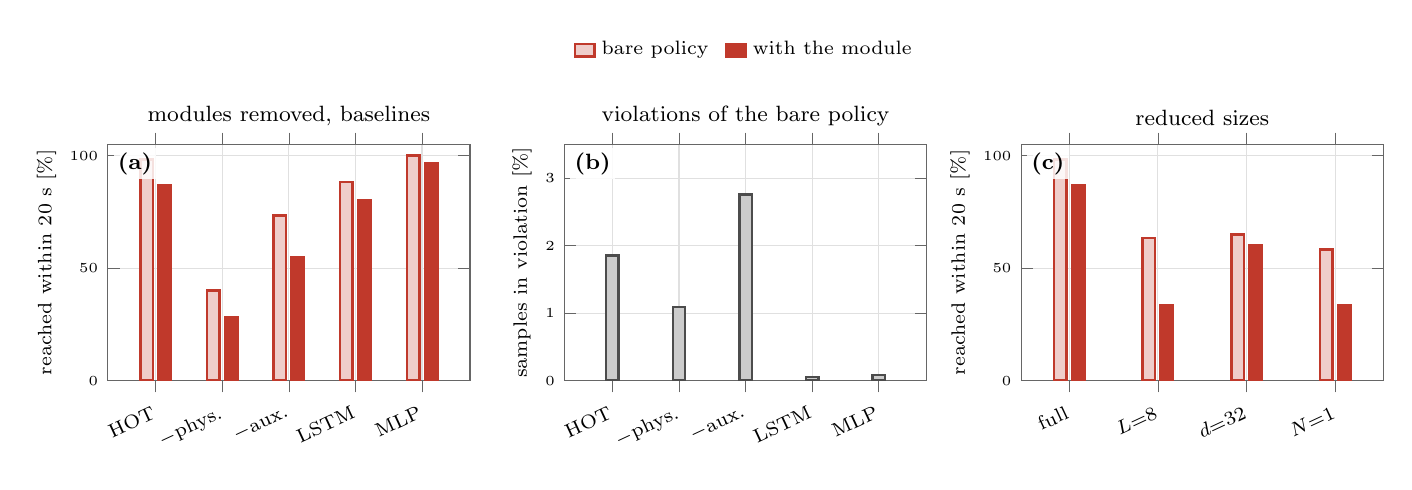
\begin{tikzpicture}
\begin{groupplot}[group style={group size=3 by 1, horizontal sep=12mm}, paperaxis, width=4.6cm, height=3.0cm, ybar, /pgf/bar width=4.5pt, tick label style={font=\tiny}, x tick label style={font=\scriptsize, rotate=25, anchor=north east}, label style={font=\scriptsize}, enlarge x limits=0.18, ymin=0]
\nextgroupplot[title={modules removed, baselines}, xtick={0,1,2,3,4}, xticklabels={HOT,$-$phys.,$-$aux.,LSTM,MLP}, ylabel={reached within 20 s [\%]}, ymax=105, legend to name=ablleg, legend columns=2, legend style={font=\scriptsize, draw=none, fill=none, /tikz/every even column/.append style={column sep=4pt}}, legend image code/.code={\draw[#1] (0cm,-0.08cm) rectangle (0.25cm,0.08cm);}]
\addplot[fill=chot!25, draw=chot] coordinates {(0,98.3) (1,40.0) (2,73.3) (3,88.3) (4,100.0)}; \addlegendentry{bare policy}
\addplot[fill=chot, draw=chot] coordinates {(0,86.7) (1,28.3) (2,55.0) (3,80.0) (4,96.7)}; \addlegendentry{with the module}
\panel{a}{}
\nextgroupplot[title={violations of the bare policy}, xtick={0,1,2,3,4}, xticklabels={HOT,$-$phys.,$-$aux.,LSTM,MLP}, ylabel={samples in violation [\%]}, ymax=3.5]
\addplot[fill=black!20, draw=black!70] coordinates {(0,1.85) (1,1.09) (2,2.76) (3,0.05) (4,0.08)};
\panel{b}{}
\nextgroupplot[title={reduced sizes}, xtick={0,1,2,3}, xticklabels={full,$L{=}8$,$d{=}32$,$N{=}1$}, ylabel={reached within 20 s [\%]}, ymax=105]
\addplot[fill=chot!25, draw=chot] coordinates {(0,98.3) (1,63.3) (2,65.0) (3,58.3)};
\addplot[fill=chot, draw=chot] coordinates {(0,86.7) (1,33.3) (2,60.0) (3,33.3)};
\panel{c}{}
\end{groupplot}
\node[anchor=south, inner sep=1pt] at ($(group c1r1.north west)!0.5!(group c3r1.north east)+(0,9mm)$) {\pgfplotslegendfromname{ablleg}};
\end{tikzpicture}
\end{document}